\documentclass[12pt,a4paper,utf8x]{report}
\usepackage [frenchb]{babel}
\usepackage[utf8]{inputenc}  
\usepackage[T1]{fontenc} 
% Pour pouvoir utiliser 
\usepackage{ucs}
\usepackage{textcomp}
\usepackage{graphicx}
\usepackage{keystroke}
\usepackage{amssymb}
\usepackage{amsmath}
%\usepackage{pifont}
\usepackage{url} % Pour avoir de belles url
\usepackage{geometry}
\usepackage{hyperref}


\usepackage {listings}% Pour mettre du code source
\lstset{language=sh}

% Pour pouvoir passer en paysage
\usepackage{lscape}

% Pour pouvoir faire plusieurs colonnes
\usepackage {multicol}

\usepackage{makeidx}% Pour crééer un index
\usepackage{graphicx} % Pour insérer des images (entres autres)
\usepackage{fourier-orns} %logo comme \danger
\usepackage[cc]{titlepic} %rajouter le logo 	 dans la page de garde
\usepackage{tocbibind}
\usepackage{wasysym} %emoticones
\usepackage{glossaries} % Créer un glossaire
\hypersetup{
  backref=true,
  %permet d'ajouter des liens dans...
  pagebackref=true,%...les bibliographies
  hyperindex=true, %ajoute des liens dans les index.
  colorlinks=true, %colorise les liens
  breaklinks=true, %permet le retour à la ligne dans les liens trop longs
  urlcolor= blue, %couleur des hyperliens
  bookmarks=true, %créé des signets pour Acrobat
  bookmarksopen=true,
  %si les signets Acrobat sont créés,
  %les afficher complètement.
  pdftitle={MiniP1_rapport}, %informations apparaissant dans
  pdfauthor={MARGUERITE Alain\\ RINCE Romain},
  %dans les informations du document
  pdfsubject={LoCD}
  %sous Acrobat.
}
%Entête pied de page
%Définition des entêtes : 
\usepackage{fancyhdr}
\pagestyle{fancy}

\lstset{language=XML,    numbers=left
   , tabsize=2
   , frame=single
   , breaklines=true
   , basicstyle=\ttfamily
   , numberstyle=\tiny\ttfamily
   , framexleftmargin=13mm
   , xleftmargin=12mm
   %, frameround={tttt}
   , captionpos=b  }
%\usepackage{pifont}
\usepackage[cc]{titlepic}
\usepackage{url} % Pour avoir de belles url
\usepackage {geometry}

% Pour mettre du code source
\usepackage {listings}
% Pour pouvoir passer en paysage
\usepackage{lscape}

% Pour pouvoir faire plusieurs colonnes
\usepackage {multicol}
% POur crééer un index
\usepackage{makeidx}
\usepackage{graphicx}
\makeindex

% Pour l'interligne de 1.5
\usepackage {setspace}
% Pour les marges de la page
\geometry{a4paper, top=2.5cm, bottom=3.5cm, left=1.5cm, right=1.5cm, marginparwidth=1.2cm}

\parskip=5pt %% distance entre § (paragraphe)
\sloppy %% respecter toujours la marge de droite 

% Pour les pénalités :
\interfootnotelinepenalty=150 %note de bas de page
\widowpenalty=150 %% veuves et orphelines
\clubpenalty=150 

%Pour la longueur de l'indentation des paragraphes
\setlength{\parindent}{15mm}



%%%% debut macro pour enlever le nom chapitre %%%%
\makeatletter
\def\@makechapterhead#1{%
  \vspace*{50\p@}%
  {\parindent \z@ \raggedright \normalfont
    \interlinepenalty\@M
    \ifnum \c@secnumdepth >\m@ne
        \Huge\bfseries \thechapter\quad
    \fi
    \Huge \bfseries #1\par\nobreak
    \vskip 40\p@
  }}

\def\@makeschapterhead#1{%
  \vspace*{50\p@}%
  {\parindent \z@ \raggedright
    \normalfont
    \interlinepenalty\@M
    \Huge \bfseries  #1\par\nobreak
    \vskip 40\p@
  }}
\makeatother
%%%% fin macro %%%%

%Couverture 



\title
{
	\normalsize{ M1 ALMA\\ 
	Université de Nantes\\
	2010-2011}\\
	\vspace{15mm}
	\Huge{Projet de Travaux pratiques :\\Systèmes Distribués \\ Mini -projet1}
}



\author{MARGUERITE Alain\\ RINCE Romain
	\vspace{45mm}
}
\titlepic{
\includegraphics[scale=1.70]{img/logouniv}     \hspace{2cm} 
\includegraphics[scale=0.12	]{img/logo}}
\date
{	
	\normalsize{Université de Nantes \\ 2 rue de la Houssinière, BP92208, F-44322 Nantes cedex 03, FRANCE
	\\ 
	\vspace{5mm}	
	Encadrant : QUEUDET Audrey \\
	}
}
\newglossaryentry{unix}{name=Unix,description={Le système Unix est un système d'exploitation multi-utilisateurs, multi-tâches, ce qui signifie qu'il permet à un ordinateur mono ou multi-processeurs de faire exécuter simultanément plusieurs programmes par un ou plusieurs utilisateurs. }}

\begin{document}
\renewcommand{\labelitemi}{$\bullet$} 	
\maketitle


\clearpage

\tableofcontents
\clearpage

% Pour avoir un interligne de 1,5
\begin{onehalfspace}
\chapter{Cahier des charges}
\paragraph{Introduction :}
 L'objectif est de définir un outil de simulation  d'ordonnancement de tâches en temps réel. Parmi ses fonctionnalités, l'outil devra pour tester les contraintes temporelles d'un ensemble de tâches générées au préalable. La génération de ces tâches entre dans la conception de l'outil. Cet outil permettra d'exporter le résultat dans un fichier  d'extension $.ktr$ pour être exploité directement par l'outil graphique Kiwi.
 
\section{Données en entrées}
L'outil doit pouvoir permettre à l'utilisateur de rentrer des tâches périodiques et ou apériodiques lui même (en précisant chacun des attributs) ou de demander une génération aléatoire pour les deux catégories.
\section{Fonctionnement}
\begin{itemize}
\item
Une analyse d'ordonnançabilité. L'outil affichera à l'utilisateur les résultats des différents tests avec les conclusions qui en découlent.
\item
Un environnement de simulation. L'outil lors du calcul de l'ordonnancement devra afficher les différents événements. Un bilan de ces action sera résumé dans un fichier au terme de l'exécution (facultatif).

L'outil doit pouvoir proposer plusieurs politiques d'ordonnancement. \`A savoir : 
\begin{itemize}
\item
Pour les tâches périodiques :

\begin{itemize}
\item
Rate Monotonic
\item
EDF
\end{itemize}

\item
Pour les tâches apériodiques : 
\begin{itemize}
\item
BG
\item
TBS
\end{itemize}

\end{itemize} 
\item
Un fichier d'extension $.ktr$ sera généré au terme de l'exécution, et contiendra le déroulement de l'ordonnancement jusqu'à'a son terme.
\item
L'outil doit communiquer, au terme de l'exécution, différents résultats de performance qu'il aura lui même calculés. Les informations à fournir sont les suivantes : 
\begin{itemize}
\item
Le nombre de violations d'échéances.
\item
Le nombre de commutations de contexte et de préemptions.
\end{itemize}
\end{itemize}


\chapter{Analyse et solution du problème}
\chaptermark{Analyse}

\section{Introduction et choix du langage}
Dans le cadre du module Systèmes Distribués, l'opportunité de  spécifier et concevoir  un générateur de tâches temps réel nous est proposé. Le langage d'implémentation étant libre, notre binôme a opté pour Java. Ce choix est basé principalement par le fait qu'il s'agissait du langage le mieux maitrisé. Cela nous a permis de concentrer nos efforts sur la mise en place des algorithmes et non sur des problèmes de langage.
 L'objectif est de définir un outil de simulation  d'ordonnancement de tâches en temps réel.

\section{Modélisation du problème}
Suite à l'étude du cahier des charges nous proposons l'architecture de l'outil suivante :
   \begin{figure}[htbp]
  \centering
  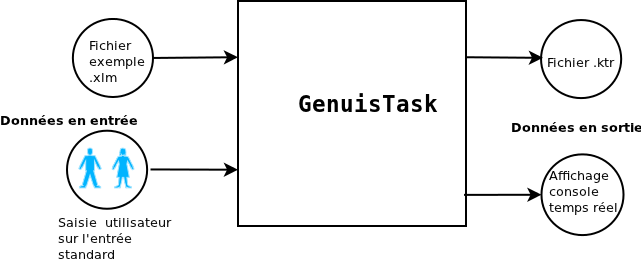
\includegraphics[scale=0.70]{img/archi}
  \caption{Architecture de l'outil}
  \label{fig:archi}
\end{figure}
\section[Génération de tâches dans un fichier]{Génération de tâches dans un fichier%
\sectionmark{Génération fichier}}
\sectionmark{Génération fichier}
La première partie du projet avait pour objectif d'obtenir un nombre $n$ de tâches périodiques et apériodiques pour de futurs traitements décrits dans la seconde partie (\ref{Part2}). \`A nouveau le choix du format d'un tel fichier nous était laissé. Nous avons choisi de générer un fichier xml (à nouveau pour des raisons  de simplicité) à la syntaxe suivante : 

\begin{itemize}
\item
Des balises \verb+<genTache.AbstractTache-array>+ encadrent la totalité du fichier.
\item
Une tâche périodique sera définie dans une balise  \verb+<genTache.TachePeriodique>+ 
\item
Une tâche apériodique sera définie dans une balise  \verb+<genTache.TacheAPeriodique>+ 
\item
Dans une tâche tous ses attributs seront définis de la manière suivante \verb+<nom_attribut>valeur_attribut</nom_attribut>+
\end{itemize}

Voici un exemple d'un fichier respectant le format décrit ci-dessus : 

\begin{lstlisting}
<genTache.AbstractTache-array>
  <genTache.TachePeriodique>
    <Pi>377</Pi>
    <ri>0</ri>
    <id>1</id>
    <Ci>1</Ci>
    <Di>1</Di>
  </genTache.TachePeriodique>
  <genTache.TachePeriodique>
    <Pi>162</Pi>
    <ri>0</ri>
    <id>2</id>
    <Ci>6</Ci>
    <Di>30</Di>
  </genTache.TachePeriodique>
  <genTache.TacheAperiodique>
    <ri>859</ri>
    <id>3</id>
    <Ci>26</Ci>
    <Di>71</Di>
  </genTache.TacheAperiodique>
</genTache.AbstractTache-array>
\end{lstlisting}
On remarque que les taches périodiques sont identifiées par : 
\begin{itemize}
\item
Pi : période d'activation.
\item
ri : date de réveil.
\item
id : L'id de la tâche.
\item
Ci : durée d'exécution maximale.
\item
Di  : délai critique
\end{itemize} 
Alors que les tâches apériodiques ont seulement : 
\begin{itemize}
\item
ri  : date de réveil
\item
id : L'id de la tâche.
\item
Ci : durée d'exécution maximale.
\item
Di : délai critique.
\end{itemize} 



\section[Algorithmes]{Algorithmes et structures mises en œuvre%
\sectionmark{Algorithmes}}
\sectionmark{Algorithmes}


\subsection{Commentaires sur la première Partie}
   \begin{figure}[htbp]
  \centering
  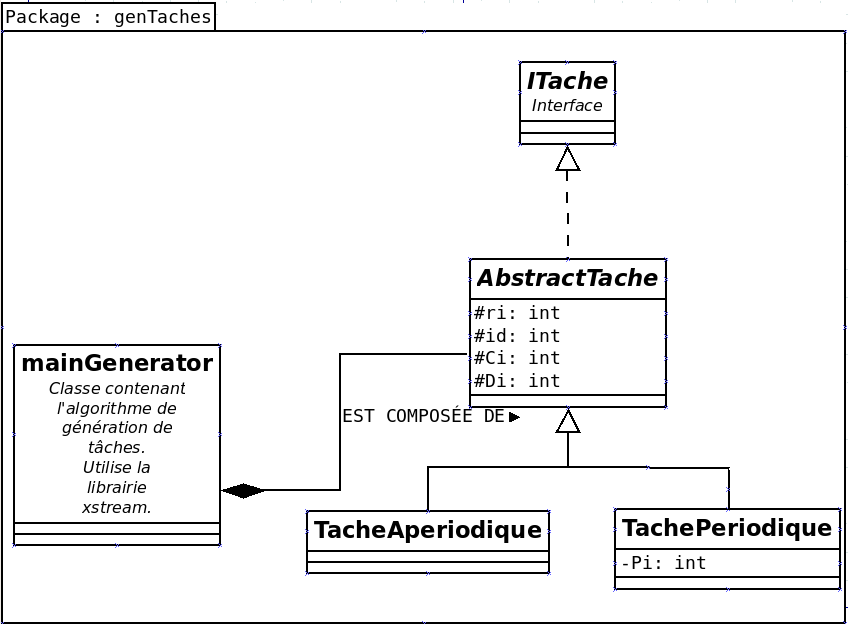
\includegraphics[scale=0.60]{img/packgen}
  \caption{Package générateur de tâches temps réel}
  \label{fig:gen}
\end{figure}

\paragraph{Calcul des tâches apériodiques} 
Le calcul des tâches ap est effectué selon la formule suivante : $ U_a =  \frac{\sum_{i=1}^m C_i}{ppcm(P_i)}$. L'utilisateur entre la variable Uap  et le nombre de tâches apériodiques qu'il désire. 
\paragraph{Détail sur la génération aléatoire}\label{PremPart}
Le cahier des charges spécifiait que la génération se devait d'offrir la possibilité de générer les tâches aléatoirement ou bien en laissant l'utilisateur choisir les paramètres de chacune d'elle. Cependant la génération de tâches aléatoires pose de nombreux problèmes.

Le premier problème est de savoir qu'elle est la taille maximale que l'on peut attribué a un $Ci$ ou un $Pi$. Il aurait été possible de laisser le choix à l'utilisateur mais dès que le nombre de tâches dépasse deux ou que leur $Pi$ est grand, l'hyperpériode explose. L'objectif étant par la suite de pouvoir générer un fichier pour kiwi, il est assez gênant d'avoir des durées d'ordonnancements qui dépassent les possibilités des valeurs pour kiwi.

Un autre problème étant de savoir comment générer les tâches pour offrir une palette large vis-à-vis des propriétés des tâches.

Au final le programme de génération des tâches aléatoires est peu sûr et laisse la possibilité, à l'utilisateur, d'entrer des informations contradictoires qui peuvent, dans la majorité des cas, faire échouer la génération.
Par exemple l'utilisateur peut rentrer un nombre de tâches apériodiques non nulle mais mettre ensuite une utilisation processeur nulle pour ces mêmes tâches, ayant pour conséquence de retourner une erreur lors de la génération.

\subsection{Deuxième partie}\label{Part2}
La deuxième partie du projet, consistait à partir du fichier de tâches (cf Première Partie), de créer un simulateur proposant  deux types de fonctionnalités :
\begin{itemize}
\item
une analyse d'ordonnançabilité,
\item
un environnement de simulation.
\end{itemize}
Le premier sujet de réflexion était de savoir dans quelles structures de données stocker les tâches et par quels moyens. Le choix des ArrayList s'est fait naturellement grâce en premier lieu à sa facilité de manipulation. Par ailleurs la fonctionnalité de la bibliothèque xtream permettant d'extraire le contenu d'un fichier xml dans une ArrayList en quelques lignes nous a d'd'emblée convaincue. Une fois cette première difficulté franchie une seconde de taille est apparue. Nous avons compris qu'il serait délicat de modifier directement les tâches dans les ArrayList. Notre idée initiale était de  modifier le Ci d'une  tâche après son traitement dans l'algorithme. Ce qui dans le cas des tâches périodiques par exemple, serait problématique. En effet par définition les taches périodiques  sont susceptibles  d'être traitées à plusieurs reprises. Il faut donc garder leurs propriétés initiales intactes. Nous avons donc choisi d'organiser notre programmation en plusieurs classes pour bien séparer les opérations de manipulation des données d'une part, les opérations mettant en jeux les algorithmes d'ordonnancement et enfin celles écrivant dans le fichier de sortie au format .ktr

   \begin{figure}[htbp]
  \centering
  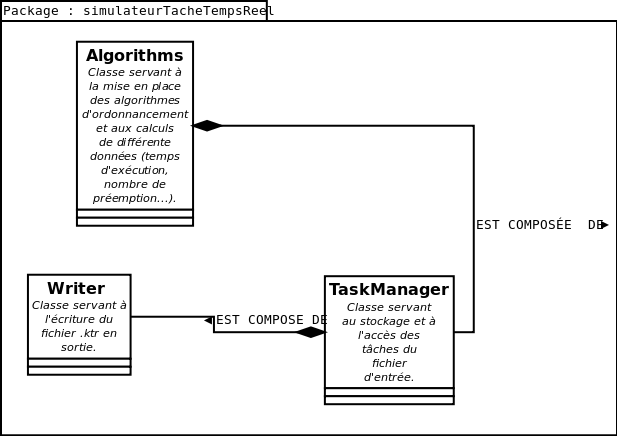
\includegraphics[scale=0.70]{img/packsstr}
  \caption{Package : Simulateur de systèmes temps réel}
  \label{fig:sstr}
\end{figure}
%\clearpage
\section{Interface proposée}
Toutes l'interface de l'outil est en ligne de commande. L'absence d'IHM graphique est due au manque de temps et au peu d'intérêt que cela représentait pour le problème étudié. De même l'outil ne prend en compte aucune option. Même si cet aspect aurait apporté un certain confort à l'utilisateur, nous avons opté pour la solution de lui demandé au fur et à mesure de l'exécution du programme les diverses options et paramètres requis. Nous avons regretté ce choix lors de la phase des tests (la répétition sans cesse des divers options est fastidieuse). Cependant nous avons gagné un temps de conception non négligeable. 



\chapter{Manuel utilisateur}
%
\includegraphics[scale=0.10]{img/logo}
\begin{figure}[htbp]
  \centering
  
\includegraphics[scale=0.10]{img/logo}

\end{figure}
%\section{Introduction et objectifs}
\label{chap:fichDonnees}
\subsection{Avis au lecteur} 
Ce manuel est destiné à un public désirant utiliser le logiciel GT. C'est à dire depuis son installation jusqu'à la génération du fichier au d'un fichier au format .ktr.Le manuel n'a pas pour objectif d'enseigner l'utilisation de cet outil. Les auteurs recommandes l'ouvrage suivant pour un tel apprentissage : \cite{kiwi}.

\subsection{Présentation du logiciel GT}
GT permet la génération automatique ou manuel de de systèmes temps réel.  L'outil est dédié est uniquement utilisable en mode console.

%\section{Votre première simulation}
\sectionmark{1\up{ère} sim}
\subsection{Introduction}
Ce chapitre va vous permettre de réaliser une vote premierès simulation pour la validation de systèmes temps réel en moins de 2 minutes  \smiley ! Voici le résultat que vous obtiendrez au terme : 
\begin{figure}[htbp]
  \centering
 % 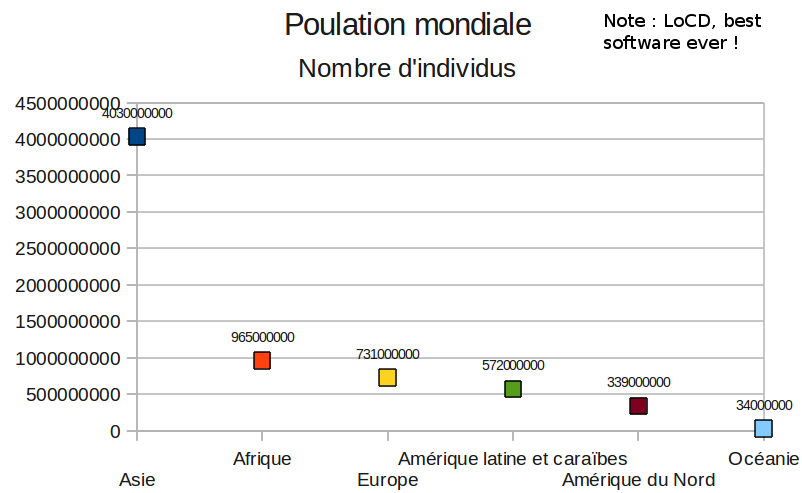
\includegraphics[scale=0.60]{img/diagrammenuages}
  \caption{Fichier .ktr}
  \label{fig:dnuages}
\end{figure}

\subsection{1\up{ère} \'Etape : Génération des tâches avec GT} 
\index{Comment commencer}
Dans le dossier GT, entrez la commande suivante \verb+./GT+. On vous propose d'entrez un nom de fichier. Entrez un nouveau nom si vous voulez créer vos propres tâches, ou entrez cours\_RMBG si vous voulez utiliser un exemple déjà éxistant. Il vous sera  demandé par la suite quel type d'ordonnancement vous désirez utiliser. Tapez R pour Rate Monotonic-Background. 

\subsection{2\up{ème} \'Etape : Utilisation de Kiwi}
Placez vous dans le dossier ou est installé Kiwi. Tapez la commande suivante  : \verb+./kiwi &+. Une fois dans l'interface de Kiwi, cliquez sur Open. Allez ouvrir votre fichier .ktr se trouvant dans le dossier ou est installé GT. Cliquez sur l'îcone Play. Voila ce que vous obtenez :  
\begin{figure}[htbp]
  \centering
 % 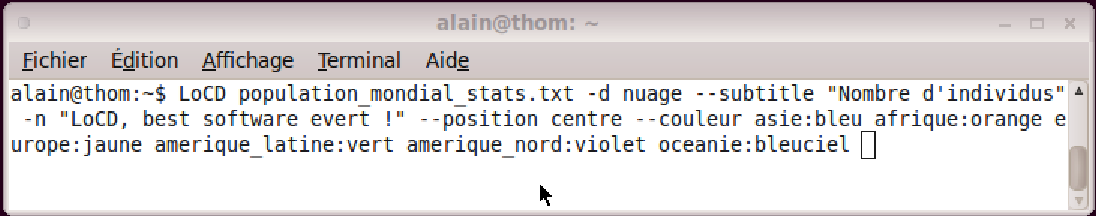
\includegraphics[scale=0.40]{img/ecommandes}
  \caption{Exemple d'utilisation de GT}
  \label{fig:commandes}
\end{figure} 


Et voilà avez crée votre première simulation pour la d'un systèmes temps réel  ! Si vous avez rencontrez des difficultés au cours de ce chapitre, vous pouvez vous référer aux différentes parties de ne manuel qui détaille chaque étapes en détail.
 
%\section{Installation et configuration}

\subsection{Configuration nécessaire}
\label{sec:conf}
\index{Configuration requise}
\danger : GT est un outil open source dédié uniquement aux systèmes d'exploitation linux. Il n'existe pas encore de version pour Windows et MAC OS. L'installation requière des connaissances dans la manipulation de commandes shell. L'ouvrage suivant est une référence dans ce domaine : \cite{Nutshell}    

\subsection{Installation}
\label{sec:install}
Rendez vous sur \url{http://www.GT.org}. La rubrique «Download» vous proposera une archive de type tar.gz pour différentes distributions (solaris, Linux 32 Bit, Linux 64 Bit, \dots ). Le téléchargement terminé, décompressez l'archive dans le dossier où vous désirez installer GT. Placez vous dans ce dossier et tapez la commande \verb+java -jar GT+. GT est maintenant installé sur votre ordinateur \smiley !!  




%\chapter{Utilisation console}
 
LoCD peut être utilisé uniquement en ligne de commande. Cette partie demandes des connaissances pré requises sur les commandes unix. En effet seul les fonctionalités de l'outil seront explicitées. La mecanisme des options est similaire à toute autres commandes unix. Pour plus de d'information sur les commandes unix, nous recommandons l'ouvrage suivant : \cite{linux}
%%%%%%%%%%%%%%%%%%%%%%%%%%%%%%%%%%%%%%%%%%%%%%%%%%%%%%%%%%%%%%%%%%%%%%
\section{Utilisation basique}
\label{sec:usebas}
La simple commande suivante générera un pdf avec d'un histogrammes avec les paramètres par défaut : % rajouter ref!!!!
\begin{verbatim}LoCD inputfile.txt\end{verbatim}Les choix du type de diagramme est possible grâce à l'option \verb+-t+ (ou \verb+--type+ ) suivit de : 
\begin{itemize}
\item
\verb+circulaire+ pour un diagramme circulaire.
\item
\verb+histogramme+ pour un histogramme.
\item
\verb+nuage+ pour un diagramme en nuage de points.
\end{itemize}
%%%%%%%%%%%%%%%%%%%%%%%%%%%%%%%%%%%%%%%%%%%%%%%%%%%%%%%%%%%%%%%%%%%%%%%%%%%%%%%%%%%%%%%%%%
\section{Gestion des méta données}
Une option pour chacune des méta données disponible (cf : ~\ref{chap:fichDonnees}) est définie :
\begin{itemize}
\item
\verb+-t+ ou \verb+--title+ pour afficher le titre.
\item
\verb+-s+ ou \verb+--subtitle+ pour afficher le sous titre.
\item
\verb+-n+ ou \verb+--note+ pour afficher le sous titre.
\end{itemize}
Si une de ces options est renseignée, il est possible de rajouter une valeur pour le paramêtre concerné. Par exemple : 
\begin{verbatim}
LoCD --title "Mon titre de diagramme" --subtitle "le sous" titre"
\end{verbatim} 
Dans le cas où l'une de ces options serait rajoutée ; et que aucune valeur ne lui est attribuée (en ligne de commande ou dans le fichier d'entrée) ; un avertissement apparaîtra à l'execution. Le diagramme n'aura pas de sous titre.\label{err:optmissing} % rajouter une ref!!!
%%%%%%%%%%%%%%%%%%%%%%%%%%%%%%%%%%%%%%%%%%%%%%%%%%%%%%%%%%%%%%%%%%%%%%%%%%%%%%%%%%%%%%%%%%

\section{Mise en forme reglages divers}
Le diagramme obtenu dans le cas d'une utilisation basique (~\ref{sec:usebas}) est stocké dans le dossier courant sous le nom de \verb+new_file.pdf+ et à les caractéristiques graphiques suivantes illustrée dans la figure :  ~\ref{fig:dbatons}.\\ Le changement du nom de ficher de sortie peut être modifier en rajoutant l'option \verb+-f outfilename+ ou dans sa version longue \verb+--filename+. 
\subsection{Couleurs}
\label{subsec:couleurs}
L'option \verb+-c+ (\verb+--couleur+) permet d'éditer la couleur de chaque données. Dans cette version LoCD propose une palette de 6 couleurs :
\begin{itemize}
\item
orange
\item
rouge
\item
vert
\item
bleu
\item
bleu ciel
\item
violet
\end{itemize}
Deux méthodes sont possibles :
\begin{enumerate}
\item
Faire suivre l'option d'un nom de couleur (listées ci-dessus). Le diagramme aura alors cette unique couleur.
\item
Faire suivre l'option du nom de la donnée puis d'un «couple» nom\_donnee:couleur séparé par le caractère \verb+:+. Une ou toutes les données peuvent être ainsi précisées. Dans tout autre cas, la couleur par défaut sera appliquée.
\end{enumerate}   
\subsection{Mise en page}
\label{subsec:misepage}
Dans la configuration par défault. Le diagramme est centrée dans une page de format A4 («au centre»). Le titre et le sous titre sont placés au dessus du diagramme (au nord»). La note elle, est placée à droite de des titres («nord est»). La figure \ref{fig:dnuages} est l'illustration de cette mise en page par défaut.
 
 

%\section{Copyright}
	\paragraph{}
    Ce programme est un logiciel libre : vous pouvez le redistribuer ou
    le modifier selon les termes de la GNU General Public Licence tels
    que publiés par la Free Software Foundation : à votre choix, soit la
    version 3 de la licence, soit une version ultérieure quelle qu'elle
    soit.
	\paragraph{}
    Ce programme est distribué dans l'espoir qu'il sera utile, mais SANS
    AUCUNE GARANTIE ; sans même la garantie implicite de QUALITÉ
    MARCHANDE ou D'ADÉQUATION À UNE UTILISATION PARTICULIÈRE. Pour
    plus de détails, reportez-vous à la GNU General Public License.
	\paragraph	{}
    Vous devez avoir reçu une copie de la GNU General Public License
    avec ce programme. Si ce n'est pas le cas, consultez
 \cite{GNU}   
  \begin{figure}[htbp]
    \centering
    
\includegraphics{/home/alain/workspace/MiniP1/Rapport/img/gpl}
  \end{figure}  


\chapter{Jeux d'essais}
\section{Cas de RMBG}
L'utilisation de la combination des algorithmes Rate Monotonic et BackGround : donne  le fichier kiwi suivant : 
\begin{figure}[htbp]
  \centering
  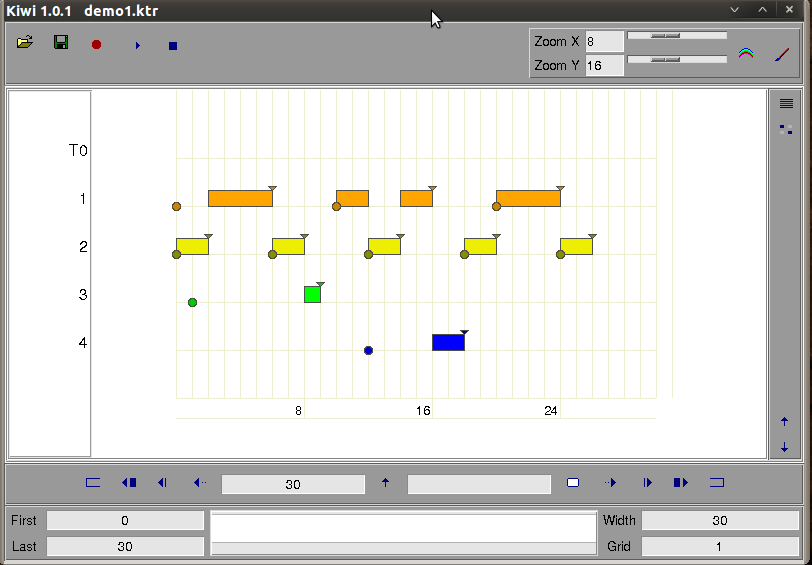
\includegraphics[scale=0.60]{img/RMBG}
  \caption{Résultat de l'appelle à RMBG}
  \label{fig:RMBG}
\end{figure}
On obtient les résultat suivants suivants : 
\begin{verbatim}
PPCM : 30
Resultat du test de faisabilité : 0.73333335

Déroulement de l'algorithme

****BILAN ET ANALYSE****
Temps d'execution : 30
Temps creux : 5
Utilisation du processeur :83
Nombre de préemptions :1
****TacheAp****
Temps de réponse min : 4
Temps de réponse max : 7
Temps de réponse moy : 6.5
\end{verbatim}
\section{Cas de EDFBG}
L'utilisation de la combination des algorithmes Earliest Deadline First et BackGround : donne  le fichier kiwi suivant : 
\begin{figure}[htbp]
  \centering
  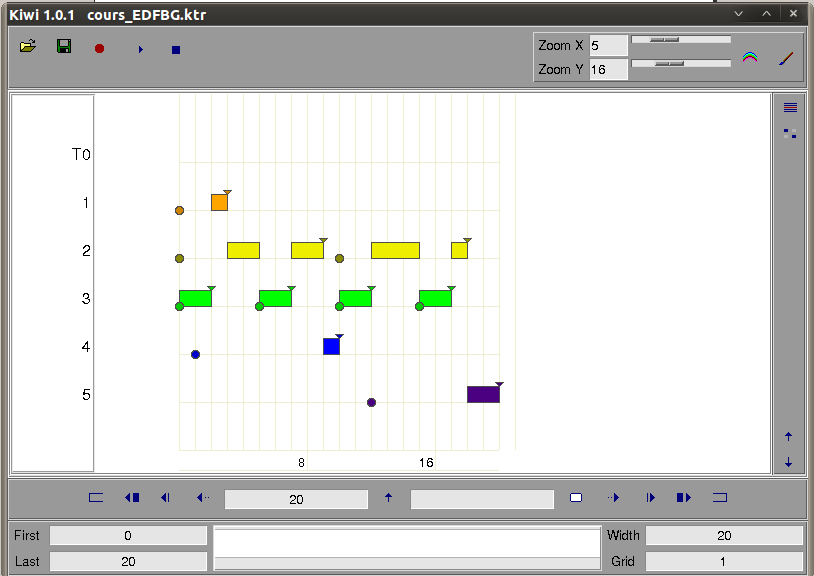
\includegraphics[scale=0.60]{img/EDFBG}
  \caption{Résultat de l'appelle à EDFBG}
  \label{fig:EDFBG}
\end{figure}
On obtient les résultat suivants suivants : 

\begin{verbatim}
Resutalt du test pour Ci<Pi selon EDF U= : 0
U<=1 condition suffisante vérifiée

Déroulement de l'algorithme

****BILAN ET ANALYSE****
Temps d'execution : 20
Temps creux : 0
Utilisation du processeur :100
Nombre de préemptions :2
****TacheAp****
Temps de réponse min : 6
Temps de réponse max : 8
Temps de réponse moy : 8.0
\end{verbatim}

\chapter{Bilan et conclusion}
parler qu'une autre structure que les ArrayList aurait été mieux.
 bilan bilan bilan bilan bilan bilan bilan bilan bilan bilan bilan bilan bilan bilan bilan bilan bilan bilan bilan bilan bilan bilan bilan bilan bilan
 bilan bilan bilan bilan bilan bilan bilan bilan bilan bilan bilan bilan bilan bilan bilan bilan bilan bilan bilan bilan bilan bilan bilan bilan bilan


% Pour finir l'interligne de 1,5
\end{onehalfspace}

\printglossary

\listoffigures

\printindex

\appendix

\bibliographystyle{alpha}
\bibliography{biblio.bib}


\end{document}
